\documentclass{article}

% if you need to pass options to natbib, use, e.g.:
%     \PassOptionsToPackage{numbers, compress}{natbib}
% before loading neurips_2024


% ready for submission
\usepackage[final]{neurips_2024}


% to compile a preprint version, e.g., for submission to arXiv, add add the
% [preprint] option:
%     \usepackage[preprint]{neurips_2024}


% to compile a camera-ready version, add the [final] option, e.g.:
%     \usepackage[final]{neurips_2024}


% to avoid loading the natbib package, add option nonatbib:
%    \usepackage[nonatbib]{neurips_2024}


\usepackage[utf8]{inputenc} % allow utf-8 input
\usepackage[T1]{fontenc}    % use 8-bit T1 fonts
\usepackage{hyperref}       % hyperlinks
\usepackage{url}            % simple URL typesetting
\usepackage{booktabs}       % professional-quality tables
\usepackage{amsfonts}       % blackboard math symbols
\usepackage{nicefrac}       % compact symbols for 1/2, etc.
\usepackage{microtype}      % microtypography
\usepackage{xcolor}         % colors
\usepackage{graphicx}


\title{Overcooked}


% The \author macro works with any number of authors. There are two commands
% used to separate the names and addresses of multiple authors: \And and \AND.
%
% Using \And between authors leaves it to LaTeX to determine where to break the
% lines. Using \AND forces a line break at that point. So, if LaTeX puts 3 of 4
% authors names on the first line, and the last on the second line, try using
% \AND instead of \And before the third author name.


\author{
  Davide  Luccioli\\
  University of Bologna\\
  \texttt{davide.luccioli@studio.unibo.it}
}

\begin{document}


\maketitle


\begin{abstract}
  This project focuses on the development and evaluation of agents for the Overcooked environment using Multi-Agent Proximal Policy Optimization (MAPPO), a state-of-the-art policy gradient method tailored for multi-agent settings. Our primary objective is to train agents that not only master individual layouts but also exhibit some generalization capabilities across different environment configurations and partner behaviours.
\end{abstract}


\section{Introduction}
Cooperative multi-agent reinforcement learning (MARL) presents a significant challenge in artificial intelligence, requiring agents to learn complex strategies to achieve shared goals. The Overcooked-AI environment \cite{overcooked}, has emerged as a prominent benchmark for fully cooperative multi-agent systems. In this environment, agents must coordinate their actions to maximize the number of soups delivered within a time limit. This environment offers an ideal test bed for developing robust and adaptive cooperative agents.

This project leverages the Multi-Agent Proximal Policy Optimization (MAPPO) algorithm to train agents for this environment. Our primary focus is to investigate the generalization capabilities of these agents when faced with variations in both the physical layout and the behaviour of their partners.

To this end, we conduct a series of experiments to systematically evaluate the agent's performance. We begin by establishing a baseline, training agents on individual layouts to assess their ability to learn in a fixed setting. We then investigate the agent's generalization capabilities by training it on multiple layouts simultaneously and testing it on unseen ones. Finally, we explore partner generalization by training the agent with a stochastic partner and evaluating its adaptability when paired with different policies. This report details our methodology and presents the results of these experiments.

\section{Methodology}
This section describes the methodology used to train an agent capable of operating in the Overcooked environment. The training process is based on the Multi-Agent Proximal Policy Optimization (MAPPO) algorithm, which is an extension of the Proximal Policy Optimization (PPO) algorithm designed for multi-agent environments. The implementation is built upon the Overcooked environment, which provides a challenging setting for cooperative multi-agent reinforcement learning tasks.

\subsection{Background}
\subsubsection{Proximal Policy Optimization}
Proximal Policy Optimization (PPO) \cite{ppo} is a policy-gradient method designed to ensure stable and efficient policy updates. It improves upon earlier approaches by optimizing a clipped surrogate objective function, constraining policy updates to a trusted region. The objective function is defined as follows:

\begin{equation}
L^{CLIP}_t = \min(\frac{\pi_\theta(a_t | s_t)}{\pi_{\theta_{old}}(a_t | s_t)} \hat{A}_t,\ clip(\frac{\pi_\theta(a_t | s_t)}{\pi_{\theta_{old}}(a_t | s_t)}, 1 - \varepsilon, 1 + \varepsilon) \hat{A}_t)
\end{equation}

where $\hat{A}_t$ is the estimated advantage at time $t$.

Due to its simplicity and effectiveness across domains, PPO has become a popular choice in reinforcement learning tasks.

\subsubsection{Multi-Agent PPO}
Multi-Agent PPO (MAPPO) \cite{mappo} is an extension of PPO for multi-agent environments. It follows the Centralized Training with Decentralized Execution (CTDE) framework, where agents have access to global information during training but act independently during execution. An actor network governs the agent's decisions based on local observations, whereas a centralized critic network evaluates the state of the environment using the joint observations of all agents. This architecture allows MAPPO to effectively learn cooperative behaviours in multi-agent settings.

\subsection{Implementation}
To address the challenges inherent in a cooperative environment such as Overcooked, we adopted the MAPPO algorithm. This choice was driven by the algorithm's strong performance in multi-agent tasks, particularly those requiring coordination and cooperation among agents. The training process is managed by a dedicated \texttt{AgentTrainer} class that manages data collection and training for the given agent. The training loop is structured as follows:

\begin{enumerate}
  \item \textbf{Data Collection}: The agent trainer collects data by executing the agent's policy in the environment for a specified number of episodes (\texttt{batch\_eps}). During each episode, it gathers observations, actions, rewards, and done flags, in separate buffers. Since the duration of each episode is fixed by the environment, we opted to define the batch size as the number of episodes,  rather than the number of steps. This ensures that each batch contains only complete episodes, simplifying data management, maintaining consistency in batch sizes and providing a more stable learning signal.

  \item \textbf{Reward Shaping}: In addition to the sparse rewards from the environment (based on delivering dishes), the training process incorporates the shaped rewards for both agents, enabling the networks to learn the intermediate steps necessary for the task. These rewards are kept separated and added to the global reward to form the training rewards, thus allowing both agents to learn the value of their actions independently, while still benefiting from the cooperation with the other agent.

  \item \textbf{Generalized Advantage Estimation (GAE)}: After collecting trajectories, the trainer computes advantages for each time step using GAE, which returns an exponentially weighted average of discounted TD-errors, controlled by the \texttt{gamma} and \texttt{lam} hyper-parameters. GAE helps reduce variance in the advantage estimates, leading to more stable policy updates.
  
  \item \textbf{Network Updates}: The agent's actor and critic networks are updated using the collected data. The updates are performed by the \texttt{PPOAgent} class, which handles all learning-related computations. For each batch of data, the networks are updated for a fixed number of iterations (\texttt{it\_updates}) to maximize data utilization, a common practice in PPO implementations.
\end{enumerate}

The \texttt{PPOAgent} employs an actor-critic architecture following a CTDE approach. The actor network outputs a probability distribution over the action space based on the agent's local observation, while the critic takes the joint observation of both agents as input and computes a single value for the state. 

Both the actor and critic networks are implemented as feed-forward neural networks inspired by the architecture used in \cite{ppo}. The input is first normalized using a Layer Normalization, a modification from the original paper to improve generalization performance, and is then passed through three hidden layers with Tanh activation functions. 

During training, the agent updates its networks in the \texttt{learn} method: The actor is optimized using a loss function that combines the PPO clipped surrogate objective with an entropy bonus to encourage exploration:

\begin{equation}
L^{actor} = \mathbb{E}_t[L^{CLIP}_t + \beta \mathcal{H}_t]
\end{equation}

where
\begin{itemize}
  \item $L^{CLIP}_t$ is the clipped surrogate objective
  \item $\mathcal{H}_t$ is the entropy of the policy at time $t$
  \item $\beta$ is a coefficient controlling the strength of the entropy regularization.
\end{itemize}

The critic network is trained to minimize the Mean Squared Error between its predicted value and the target return \( \hat{R}_t \), computed using Generalized Advantage Estimation (GAE):

\begin{equation}
L^{critic} = \mathbb{E}_t[(V(s_t) - \hat{R}_t)^2]
\end{equation}

Both networks are optimized separately using the Adam optimizer.

\subsection{Generalization Strategies}
A key objective of this project was to train an agent robust to variations in the environment layout or behaviours of other agents. To this end two different strategies were employed:

\begin{itemize}
  \item \textbf{Multi-Layout Training}: To train an agent capable of performing on different layouts, we defined a \texttt{GeneralizedOvercooked} environment wrapper selecting a random layout from a predefined list at the beginning of each episode. This approach allows the agent to experience multiple layouts during training, enabling it to learn a more generalized policy that can adapt to different configurations.
  
  \item \textbf{Partner Policy Generalization}: In an effort to improve the agent's ability to adapt to different partners, we modified the training process to include a stochastic partner policy. With a specified probability \texttt{random\_agent\_prob} one of the agents is substituted with a random agent that performs a random action 40\% of the time and remains idle for the other 60\%. This approach forces the agent to adapt to a potentially uncooperative partner, enhancing its ability to generalize across different partner policies. To ensure that the learning agent's policy is not corrupted by the random actions of its partner, we use a mask to exclude the random agent's actions and rewards from the training data during network updates.
\end{itemize}

\section{Results}

\subsection{Single Layout Performance}
To establish a baseline for the agent's performance, we first applied our training method separately to each of the five original layouts from the overcooked-ai library. This approach allows us to evaluate the agent's ability to learn a specific layout without the additional complexity of generalizing across different environments. The training was conducted for 5000 episodes for each layout, and the mean rewards obtained during training are shown in Figure \ref{fig:single_layout_rewards}.

\begin{figure}[ht]
\centering
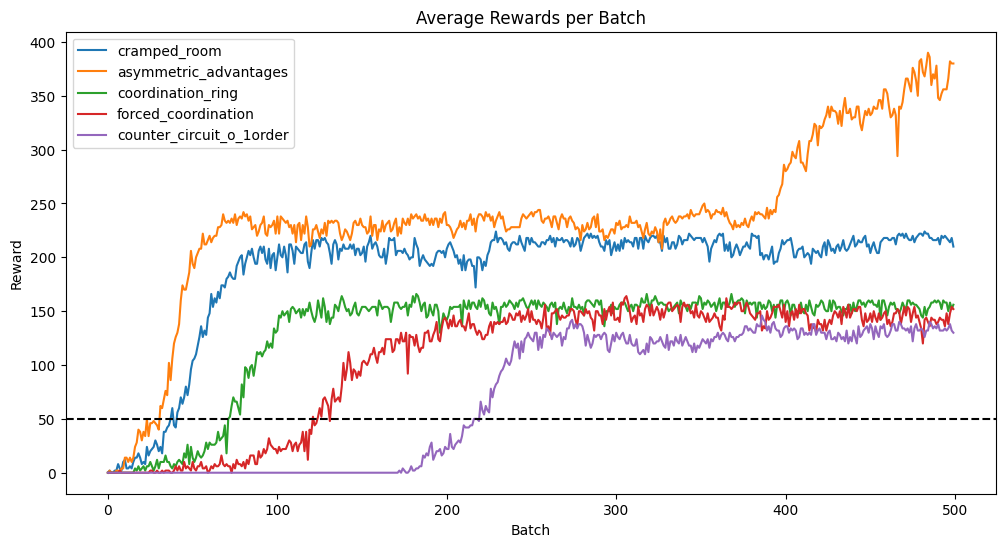
\includegraphics[width=0.75\textwidth]{../plots/mean_rewards.png}
\caption{All agents are able to learn a policy to solve the layout they were trained on, achieving higher mean rewards over time, with lower rewards and slower training for more complex layouts.}
\label{fig:single_layout_rewards}
\end{figure}

The agents' performance was evaluated by running 100 episodes in self-play mode on each layout after training. The results are summarized in Table \ref{tab:single_layout_results}.

\begin{table}[ht]
\centering
\caption{Evaluation results for single-layout training.}
\label{tab:single_layout_results}
\begin{tabular}{lccc}
\toprule
Layout & \multicolumn{1}{c}{Mean Reward} & \multicolumn{1}{c}{Std Dev} & \multicolumn{1}{c}{Mean Soups} \\
\midrule
cramped\_room & 205.0 & 9.54 & 10.25 \\
asymmetric\_advantages & 374.0 & 41.23 & 18.7 \\
coordination\_ring & 154.6 & 9.74 & 7.73 \\
forced\_coordination & 146.8 & 14.48 & 7.34 \\
counter\_circuit\_o\_1order & 133.2 & 10.67 & 6.66 \\
\bottomrule
\end{tabular}
\end{table}

The results show that for each layout the agent is able to achieve a higher mean reward than the minimum of 50 required for the \texttt{cramped\_room} layout. This indicates that the agent successfully learned to solve each layout individually, significantly exceeding the performance baseline.

Notably, the \texttt{asymmetric\_advantages} layout achieved a much higher reward due to an emergent coordination strategy where one agent, positioned closer to the ingredients, would prepare and place them in both pots, while the other agent, closer to the delivery area, would handle plating and delivering the soups.


\subsection{Multi-Layout Performance}
To evaluate the agent's ability to generalize across different environments, we trained a single agent on multiple layouts simultaneously. Based on the single-layout training results, we selected the three layouts that the agent learned most efficiently. The agent was trained for 10000 episodes, to allow all layouts to be learned effectively.

\begin{table}[ht]
\centering
\caption{Evaluation results for multi-layout training.}
\label{tab:multi_layout_results}
\begin{tabular}{lccc}
\toprule
Layout & \multicolumn{1}{c}{Mean Reward} & \multicolumn{1}{c}{Std Dev} & \multicolumn{1}{c}{Mean Soups} \\
\midrule
cramped\_room & 202.8 & 9.39 & 10.14 \\
asymmetric\_advantages & 219.6 & 15.74 & 10.98\\
coordination\_ring & 138.6 & 11.75 & 6.93 \\
simple\_o & 29.6  & 15.09 & 1.48 \\
\bottomrule
\end{tabular}
\end{table}

The agent's performance was then evaluated on all five original layouts, as well as on an additional unseen layout, \texttt{simple\_o}, which shares a similar structure to \texttt{cramped\_room}. The evaluation revealed that the agent performed well on the three layouts it was trained on. However, its performance on the more complex, unseen layouts (\texttt{forced\_coordination} and \texttt{counter\_circuit\_o\_1order}) was poor, indicating a failure to generalize to substantially different environments. Notably, the agent was able reliably deliver at least 1 soup on the \texttt{simple\_o} indicating some level of generalization on a layout with a similar structure to a known one.


\subsection{Generalization to Different Partners}
Some layouts, such as \texttt{asymmetric\_advantages}, naturally encourage specialized strategies that require close coordination between agents. If an agent learns to rely on such a strategy, its performance will suffer when paired with a partner that does not follow the expected behaviour. To address this, we trained our agent with a stochastic partner: at each training episode, one of the agents could be replaced by a random agent with a set probability, forcing the primary agent to learn how to cooperate with a less predictable player. The agents were then evaluated in self-play as well as with random and idle partners to assess their adaptability to different partner behaviours.

We re-trained agents on each layout individually for 10,000 episodes with the random partner, which showed some ability to work around the stochastic behaviour in most cases. The training was conducted with a \texttt{random\_agent\_prob} of 75\% to discourage overfitting to a coordinated policy. The \texttt{forced\_coordination} layout was excluded from this experiment, as it is unsolvable if one of the agents does not cooperate.

\begin{figure}[ht]
\centering
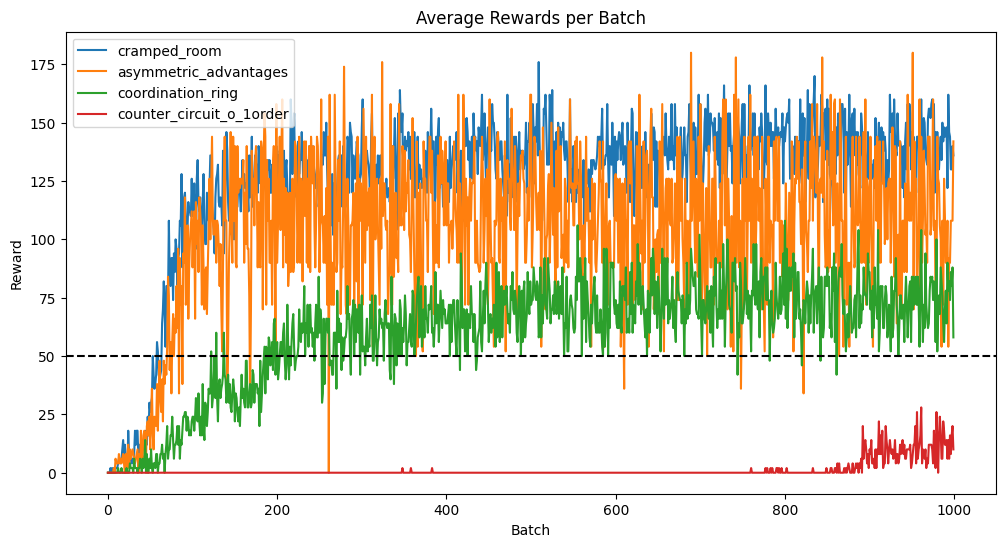
\includegraphics[width=0.7\textwidth]{../plots/mean_random_rewards.png}
\caption{Training results for partner generalization}
\label{fig:partner_generalization_rewards}
\end{figure}


As shown in table \ref{tab:partner_generalization_results}, the agent's ability to adapt to a stochastic partner varied significantly across layouts. On simpler layouts, the agents achieved better results than the self-play agent when paired with a random or idle partner, demonstrating a degree of robustness. However, this adaptability did not consistently extend to more complex layouts where specialized strategies are crucial. For instance, on \texttt{asymmetric\_advantages}, the agent's performance degraded substantially. When controlling the first player, it could manage to deliver some soups independently, but it lost its ability to coordinate, performing poorly even in self-play and making no contribution as the second player.

\begin{table}[ht]
\centering
\caption{Evaluation results for partner generalization training}
\label{tab:partner_generalization_results}
\begin{tabular}{llccc}
\toprule
Layout & Partner & Agent Pos & Mean Reward & Std Dev \\
\midrule
\textit{cramped\_room} & Self-Play & - & 185.0 & 19.7 \\
 & Random & P1 & 126.0 & 29.3 \\
 & & P2 & 130.4 & 26.7 \\
 & Idle & P1 & 150.0 & 23.0 \\
 & & P2 & N.A. & N.A. \\
\midrule
\textit{asymmetric\_advantages} & Self-Play & - & 179.6 & 2.8 \\
 & Random & P1 & 179.2 & 8.4 \\
 & & P2 & 0.6 & 3.41 \\
 & Idle & P1 & 179.8 & 3.4 \\
 & & P2 & 0.0 & 0.0 \\
\midrule
\textit{coordination\_ring} & Self-Play & - & 117.2 & 10.5 \\
 & Random & P1 & 57.0 & 20.2 \\
 & & P2 & 52.8 & 20.1 \\
 & Idle & P1 & N.A. & N.A. \\
 & & P2 & 136.8 & 7.86 \\
\midrule
\textit{counter\_circuit} & Self-Play & - & 43.6 & 14.8 \\
 & Random & P1 & 5.4 & 8.8 \\
 & & P2 & 4.4 & 8.7 \\
 & Idle & P1 & 0.0 & 0.0 \\
 & & P2 & 0.0 & 0.0 \\

\bottomrule
\end{tabular}
\end{table}

Values marked as N.A. in the table indicate that setting the partner to idle makes the task impossible to complete for that layout.

As a final test we trained a single agent on the same layouts as the multi-layout training, but with a stochastic partner. The agent was trained for 20,000 episodes with a \texttt{random\_agent\_prob} of 75\%. The results of this training were mostly comparable with those obtained by the single-layout random partner training, with the exception of the \texttt{coordination\_ring} layout, which the agent was unable to solve. 

\section{Conclusion}
The results of our experiments show that our agents are capable of learning effective policies for the Overcooked environment using the MAPPO algorithm. The agents successfully mastered individual layouts, demonstrating the ability to learn specialized strategies tailored to specific tasks. 

However, their performance on unseen layouts revealed limitations in generalization: while agents can learn to operate across a few layouts, their ability to generalize to unseen configurations remains limited. This suggests that the learned policies, while effective, are partially overfitted to the specific layouts encountered during training.

Furthermore, our experiments with a stochastic partner highlighted a trade-off between learning specialized, coordinated strategies and developing general adaptability. While agents learned to compensate for an unpredictable partner on simpler layouts, they struggled to integrate this flexibility into the highly coordinated policies required for more complex environments.

\bibliographystyle{plain}
\bibliography{biblio}
\end{document}
